
In the following, we will summarise the results obtained for the IPAC
data set. We deal with the different physical paramenters in separate
Sections. We start by reporting the cross validation Root Mean Square
Errors (RMSE) for the five-fold cross-validation strategy, and
subsequently discuss the accuracy of the predictions with respect to
literature values where available.

\subsection{Effective temperature models}

Table \ref{tab:model_IPAC_TSD} summarises the RMSE for the complete set of
models: the minimum $\chi^2$ estimate based on the full spectrum
($\chi^2$), the projection pursuit regression based on the ICA
components (PPR-ICA) and some models trained on the spectral
features proposed by the GA (GA-RF, 
GA-GBM, GA-SVR, GA-NNET, GA-MARS, GA-KPLS). For each model, we report
the RMSE obtained for several noise levels of the training sets. 
We use the following notation: RMSE represents the RMSE
obtained for a model trained and tested on BT Settl spectra. 
SNR=$\infty$ corresponds to noiseless spectra. 
The RMDSE means the root median square error, as a way to provide 
robust estimation against outliers.

Theoretical estimation about Temperature is carried out by Dr Sarro\textquoteright s 
relationship against subspectral type.

\newcommand{\ra}[1]{\renewcommand{\arraystretch}{#1}}
\begin{table*}\centering
\ra{1.3}
\begin{tabular}{@{}rrrcrrcrr@{}}\toprule
& \multicolumn{2}{c}{$SNR = 10$} & \phantom{ab}& \multicolumn{2}{c}{$SNR = 50$} &
\phantom{ab} & \multicolumn{2}{c}{$SNR = \infty$}\\
\cmidrule{2-3} \cmidrule{5-6} \cmidrule{8-9}
$Regression Models$ & $RMSE$ & $RMDSE$ && $RMSE$ & $RMDSE$ && $RMSE$ & $RMDSE$ \\ \midrule
$\chi^2 BTSettl$    &  147.48 & 79.02 && 121.40 & 55.78 && 126.03 & 57.26 \\
$ ICA+ ppr$         & 188.50 & 125.89 && 164.24 & 94.71 && 190.90 & 130.09 \\
$rf $               & 160.04 & 97.20 && 195.72 & 103.00 && 145.18 & 94.12 \\
$ gbm $             & 175.35 & 104.55 && 225.43 & 99.44 && 184.56 & 94.02 \\
$ svr $             & 203.11 & 112.06 && 284.93 & 106.29 && 367.65 & 153.64 \\
$ nnet $            & 220.97 & 83.91 && 313.43 & 111.41 && 394.81 & 202.17 \\
$ knn $             & 183.20 & 118.86 && 192.93 & 109.04 && 223.81 & 109.66  \\
$ mars+ bagging $   & 222.45 & 76.11 && 360.74 & 102.74 && 373.72 & 156.74 \\
$ kpls $            & 227.00 & 72.27 && 331.27 & 122.78 && 408.55 & 207.89 \\

\bottomrule
\end{tabular}
\caption {RMSE and RMDSE for the various regression models that predict $T_{eff}$ (K).} 
\label{tab:model_TSD} 
% \end{center}
\end{table*}


%

Most models show remarkably similar distributions of the
predictions when trained with different SNR levels. In the cases of
GA-MARS, GA-KNN, and GA-SVR this is the case even in the unrealistic
scenario of SNR=$\infty$.

In general, models tends to produce better behaved solutions (with
smaller biases and less scatter) for SNR=10. 

Major conclusion is that Temperature related features are distributed
throughout all the spectrum instead of being concetrated over specifc
bands. The reason for that is the $\chi^2$ estimator over the whole 
spectrum but the Independent Component Analysis based projections,
which behaves similarly by considering the whole spectrum.
In the same sense aproximations based on specific features performs
slightly worse that the whole spectrum, which confirms the spreaded 
features over the wavelength.

{\bf I should move this explanation to the beginning of the
section or to the methodology section.}


In Figures~\ref{fig:comp01}~\ref{fig:comp02} the relationship between Temperature
estimated from the GA technique proposed features and modeled with different 
technqiues and the $chi^2$ with SNR=50 against the 
estimations provided by Temperature estimated from 
the star\textquoteright spectral subtype can be seen.

\begin {figure}
 \centering
 \begin{subfigure}{.85\textwidth}
  \centering
  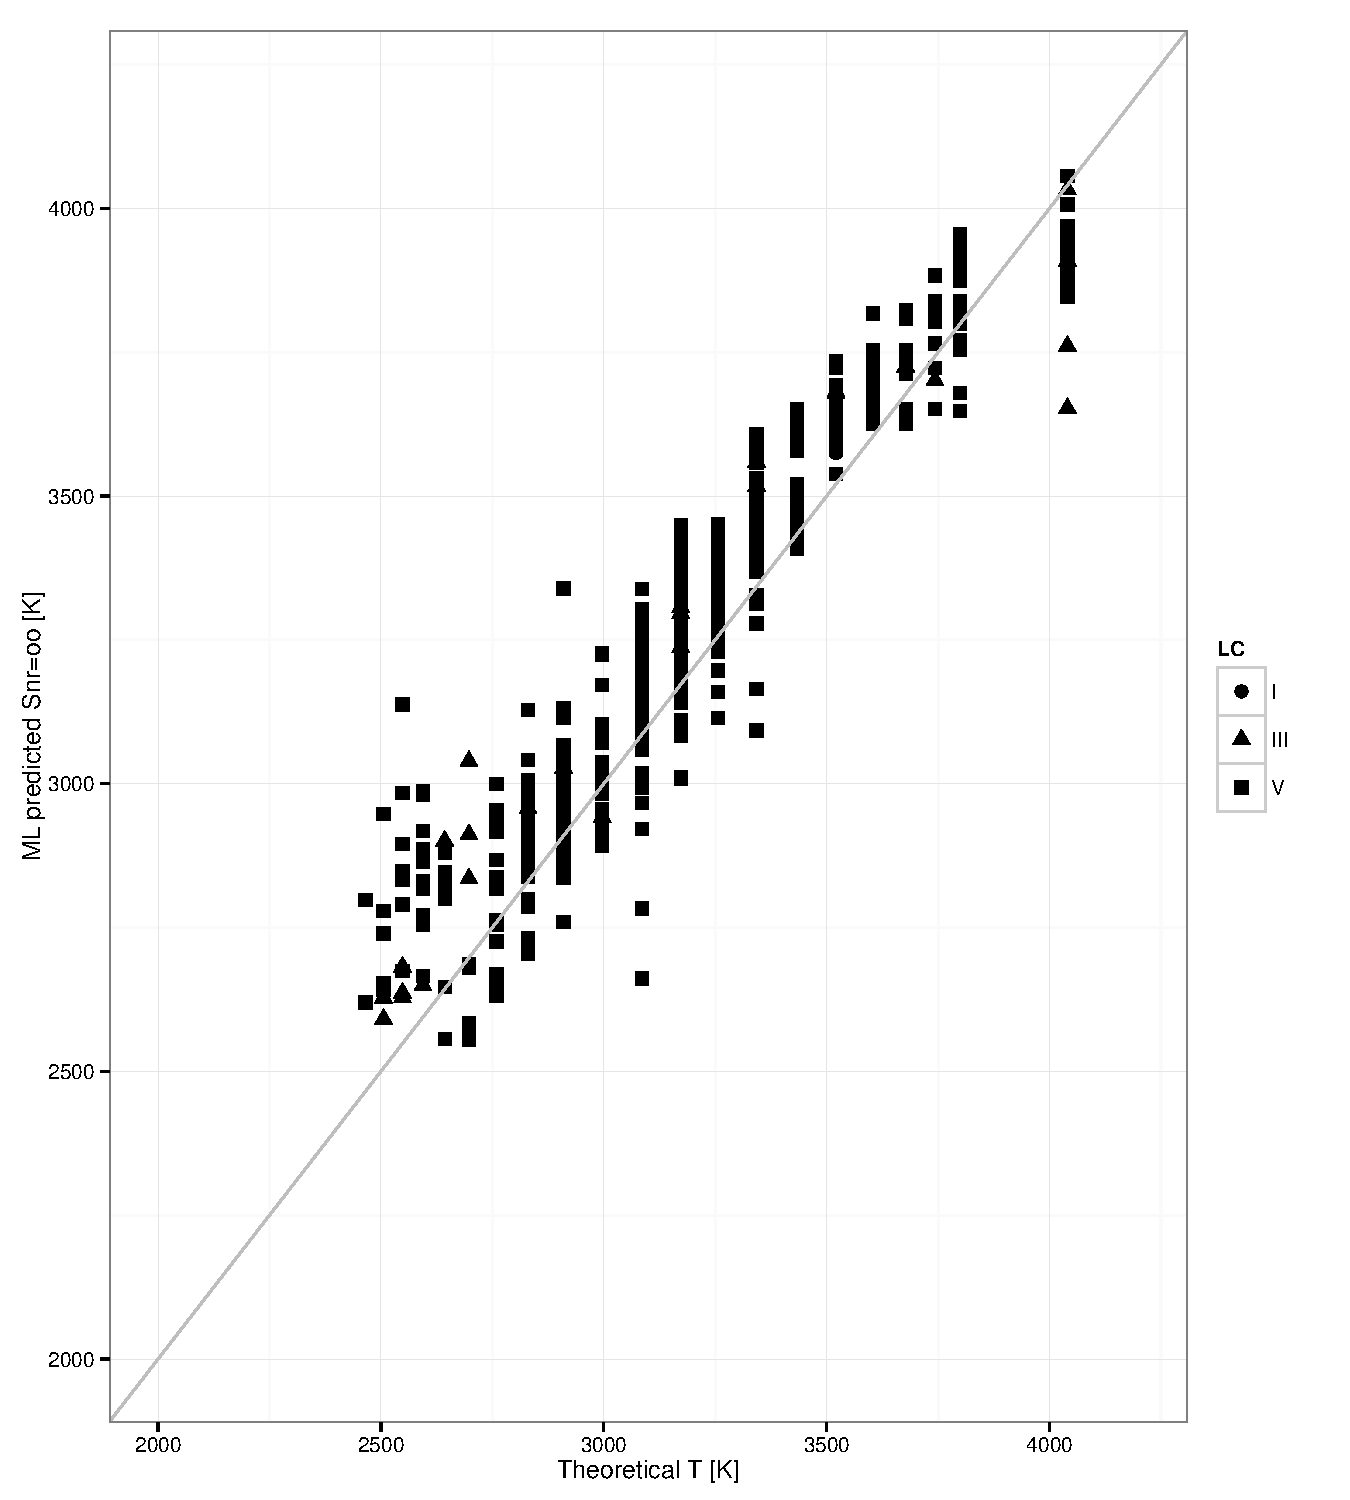
\includegraphics[width=11cm]{figs/ipac_T_ICAoo_LSB.pdf}
  \caption{Comparison between Temperature estimations from Theoretical Temperature 
  in x axis and the modeled ICA based estimation at SNR=$\infty$ on y-axis}
 \label{fig:ipac_icaoo_lsb}
 \end{subfigure}
  \begin{subfigure}{.85\textwidth}
  \centering
  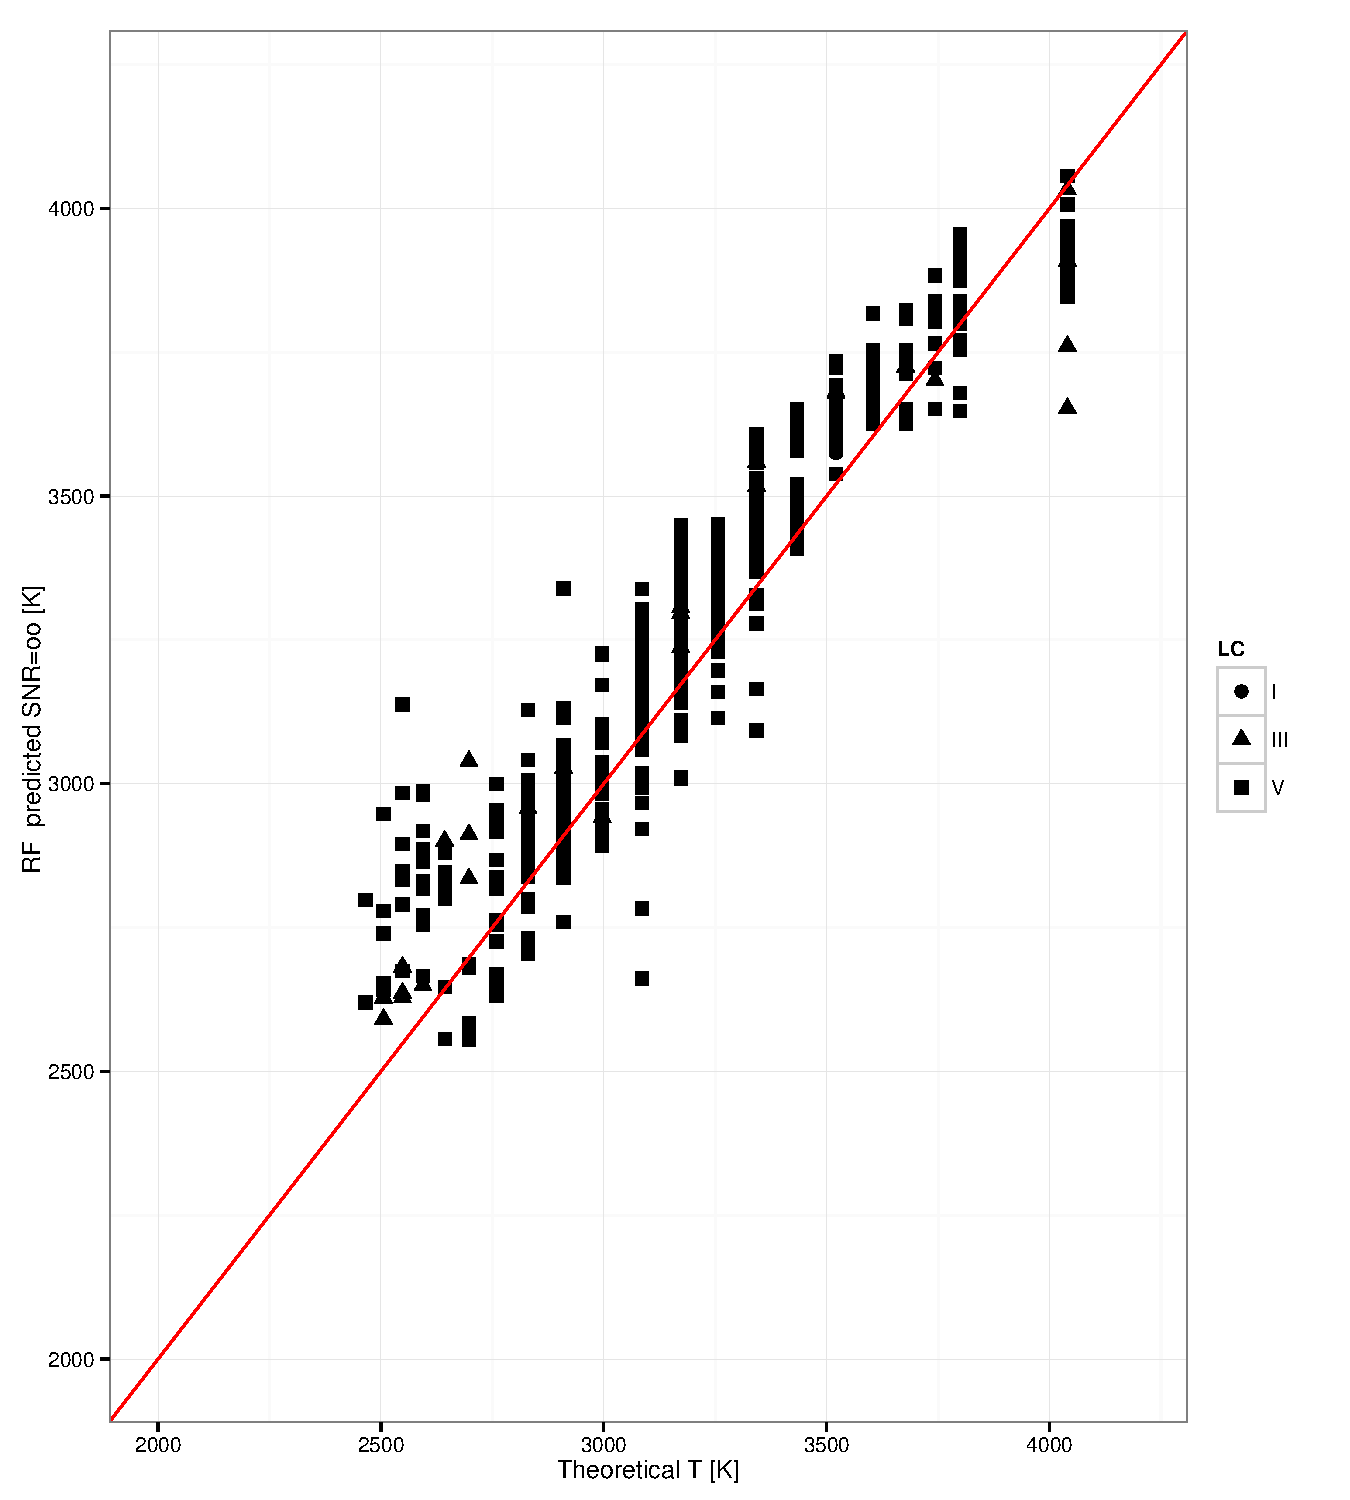
\includegraphics[width=11cm]{figs/ipac_T_RFoo_LSB.pdf}
  \caption{Comparison between Temperature estimations from Theoretical Temperature 
  in x axis and the featured based Random Forest modeled at SNR=$\infty$ on y-axis}
 \label{fig:ipac_rfoo_lsb}
 \end{subfigure}
  \begin{subfigure}{.85\textwidth}
  \centering
  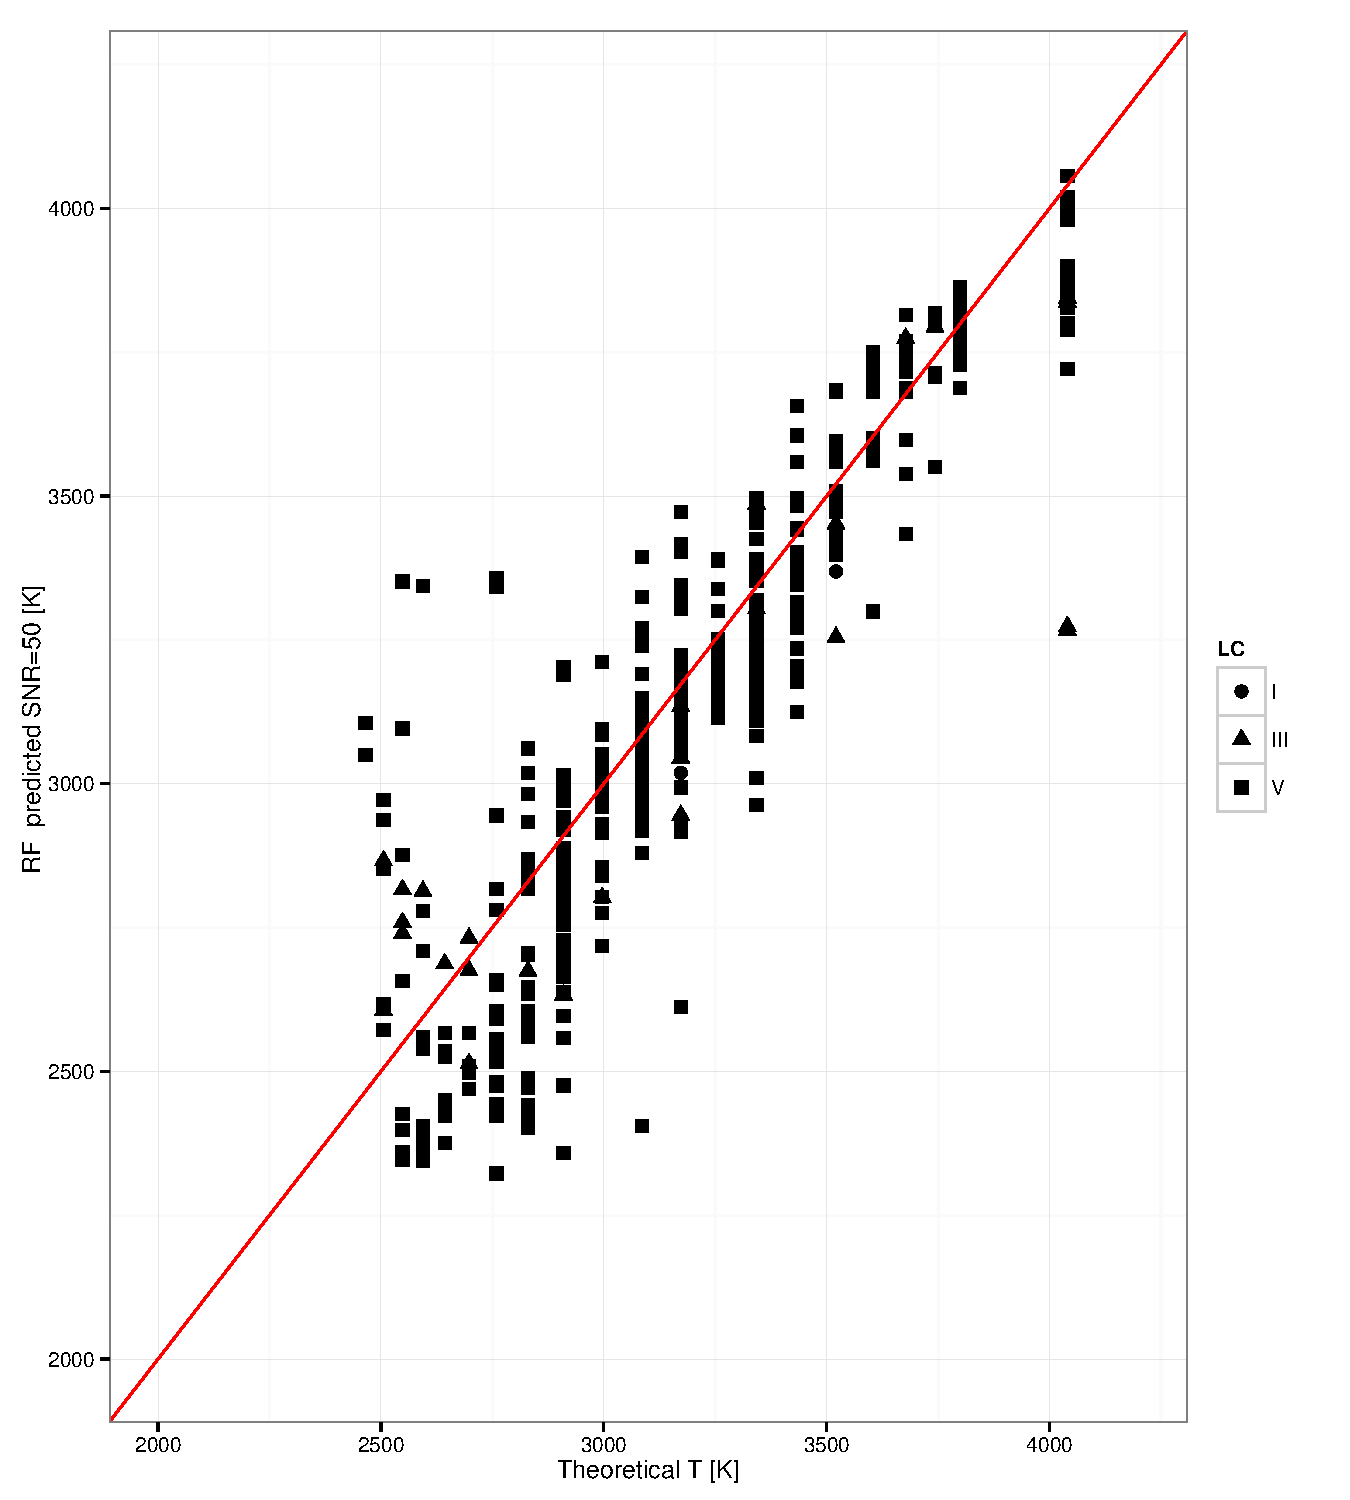
\includegraphics[width=11cm]{figs/ipac_T_RF50_LSB.pdf}
  \caption{Comparison between Temperature estimations from Theoretical Temperature 
  in x axis and the featured based Random Forest modeled at SNR=$\50$ on y-axis}
 \label{fig:ipac_rf50_lsb}
 \end{subfigure}
 \label {fig:comp01}
 \caption{Performance comparison between the different strategies for Teperature prediction}
\end {figure}
 
 
We can produce a comparison with the features provided by Cesetti, within the I band range
making sense for the IPAC spectra (see Table \ref{tab:tab_CS_T}).
\begin{table}
\begin{center}
\begin{tabular}{rrrr}
  \hline
  $\lambda_1$ & $\lambda_2$ & $\lambda_{cont;1}$ & $\lambda_{cont;2} $ \\ 
  \hline
8461 & 8474 & 8474 & 8484 \\
8484 & 8513 & 8474 & 8484 \\
8522 &  8562 & 8474 & 8484 \\
8577 & 8619 & 8563 & 8577 \\
8642 & 8682 & 8619 & 8642 \\
8730 & 8772 & 8700 & 8725 \\
8802 & 8811 & 8776 & 8792 \\
8850 & 8890 & 8815 & 8850 \\
9000 & 9030 & 8983 & 8998 \\
9080  & 9100 & 9040 & 9050 \\

\hline
\end{tabular}
\caption {Features selected by following suggestions from Cesetti et al, table 1. } 
\label{tab:tab_CS_T}
\end{center}
\end{table}

We have built nonlinear models with the same method we did for the features suggested 
by the GA techniques, learning from BT-Settl as a whole and predicting over the IPAC set
(see \ref{tab:tab_CS_Model}).

\begin{tabular}{@{}rrrcrrcrr@{}}\toprule
& \multicolumn{2}{c}{$SNR = 10$} & \phantom{ab}& \multicolumn{2}{c}{$SNR = 50$} &
\phantom{ab} & \multicolumn{2}{c}{$SNR = \infty$}\\
\cmidrule{2-3} \cmidrule{5-6} \cmidrule{8-9}
$Regression Models$ & $RMSE$ & $RMDSE$ && $RMSE$ & $RMDSE$     && $RMSE$       & $RMDSE$ \\ \midrule
$rf $               & 202.86 & 139.65 && 243.13 & 120.82 && 305.72 & 171.58  \\
$gbm $              & 187.70 & 120.04 && 160.76 & 138.07 && 336.78 & 222.11  \\
$ svr $             & 196.85 & 134.66 && 379.36 & 193.56 && 840.30 & 688.47  \\
$ nnet $            & 206.89 & 135.18 && 513.71 & 295.86 && 719.28 & 489.00  \\
$ mars+ bagging $   & 252.03 & 123.70 && 789.30 & 186.29 && 3464.16 & 784.14  \\
$knn  $             & 235.29 & 158.22 && 246.17 & 136.75 && 313.88 & 175.02  \\
$ kpls $            & 250.14 & 200.68 && 741.48 & 361.14 && 2246.74 & 1424.20  \\
$Rule Regression $  & 210.81 & 128.07 && 400.04 & 238.60 && 828.00 & 774.26  \\

\hline
\end{tabular}
\caption {Regression models performance based on Cesetti features} 
\label{tab:tab_CS_Model}
\end{center}
\end{table}



\subsection{Surface gravity models}

The same approach can become useful to produce $log(G)$ estimations. 
Here comparisons can only be possible between GA based features, the 
global spectra based approach with $\chi^2$ distance
to be minimized and those stars with gravity was 
estimated in  \cite{2013A&A...549A.129C}.

The only difference with the methodology presented above is because
Temperature has been considered a fixed feature in the estimation of 
Gravity.

In Table~\ref{tab:models_G_rmse} 
we can see the analysis of performance between
the $\chi^2$ identificacion and the one based on features from the spectrum
depending on several classes of features. The checks were carried out against 
$Log(g)$ from Rojas-Ayala.

%
% Gravedad teórica desde Cesseti para las IRTF
%
\ra{1.3}
\begin{table*}\centering
\begin{tabular}{@{}rrrcrrcrr@{}}\toprule
& \multicolumn{2}{c}{$SNR = 10$} & \phantom{ab}& \multicolumn{2}{c}{$SNR = 50$} &
\phantom{ab} & \multicolumn{2}{c}{$SNR = \infty$}\\
\cmidrule{2-3} \cmidrule{5-6} \cmidrule{8-9}
$Regression Models$ & $RMSE$ & $RMDSE$ && $RMSE$ & $RMDSE$     && $RMSE$       & $RMDSE$ \\ \midrule
$\chi^2 BTSettl$    &  2.20     & 1.62  && 2.19 & 1.49 && 2.24  & 1.56 \\
$ ICA+ ppr$         & \bf{2.14} & 1.78  && \bf{1.82} & 1.71 && 4.31  & 4.18 \\
$rf $               & \bf{1.35} & \bf{0.97} && \bf{1.62} & \bf{1.12} && \bf{1.41} & \bf{0.93} \\
$gbm $              & \bf{1.59} & \bf{1.15} && \bf{1.69} & \bf{1.37} && \bf{1.66} & \bf{1.17} \\
$ svr $             & \bf{1.98} & 1.81  && \bf{2.13} & 1.88  && 2.28 & 1.58 \\
$ nnet $            & \bf{2.03} & 1.78  && 2.25 & 1.95 && 3.22 & 2.78 \\
$ mars+ bagging $   & \bf{1.85} & \bf{1.55} && \bf{2.03} & 1.73 && \bf{2.03}  & \bf{1.50} \\
$knn  $             & \bf{2.05} & \bf{1.54} && 2.18 &  1.73  &&  \bf{1.71} & \bf{1.19} \\
$ kpls $            & \bf{1.85} & \bf{1.44} && \bf{2.01} & 1.72 && 2.75 & 2.31 \\
$Rule Regression $  & \bf{2.01} & 1.76 && \bf{2.09} & 1.80 && 3.73 &  3.22 \\

\bottomrule
\end{tabular}
\caption {RMSE and RMDSE for the various regression models predicting $Log(G)$ [dex].} 
\label{tab:models_G_rmse} 
% \end{center}
\end{table*}


It is possible to present relationships between $log(g)$ and $log(T)$
as a matter of congruence analysis between predictions. In the Figure~\ref{fig:lt_lg_ga}
such relationship is presented for models based on artificial intelligence selected features.

\begin{figure}
 \begin{center}
 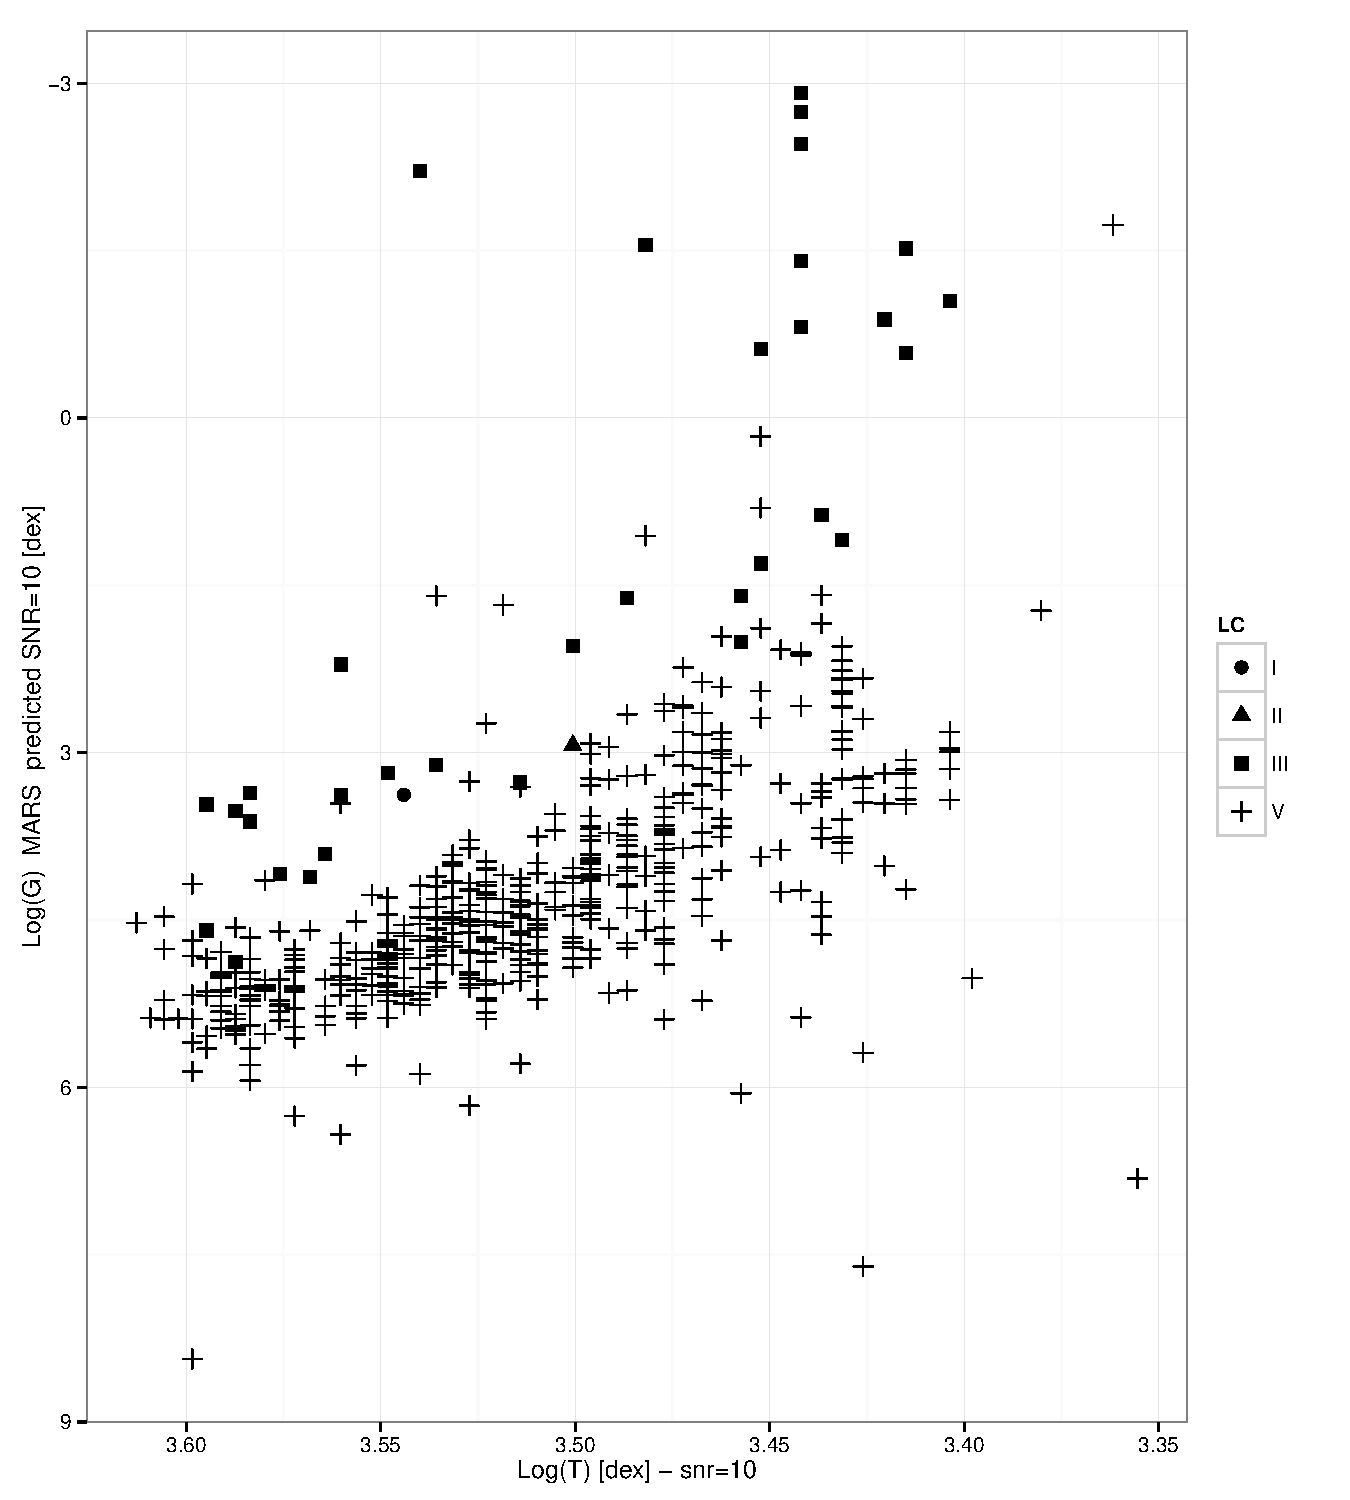
\includegraphics[width=12cm]{figs/ipac_LG_T_Mars_10.pdf}
 \caption{Relationship between $log(T) $ in the x axis 
 and $log(g)$ in the y axis for MARS model based on the GA provided bandpass features with SNR=$\10$}
 \label{fig:lt_lg_ga}
 \end{center}
\end{figure}

We can plot relationships between $log(g)$ and $log(T)$
as a matter of congruence analysis between predictions. In the Figure~\ref{fig:lt_lg_pls}
such relationship is presented.

\begin{figure}
 \begin{center}
 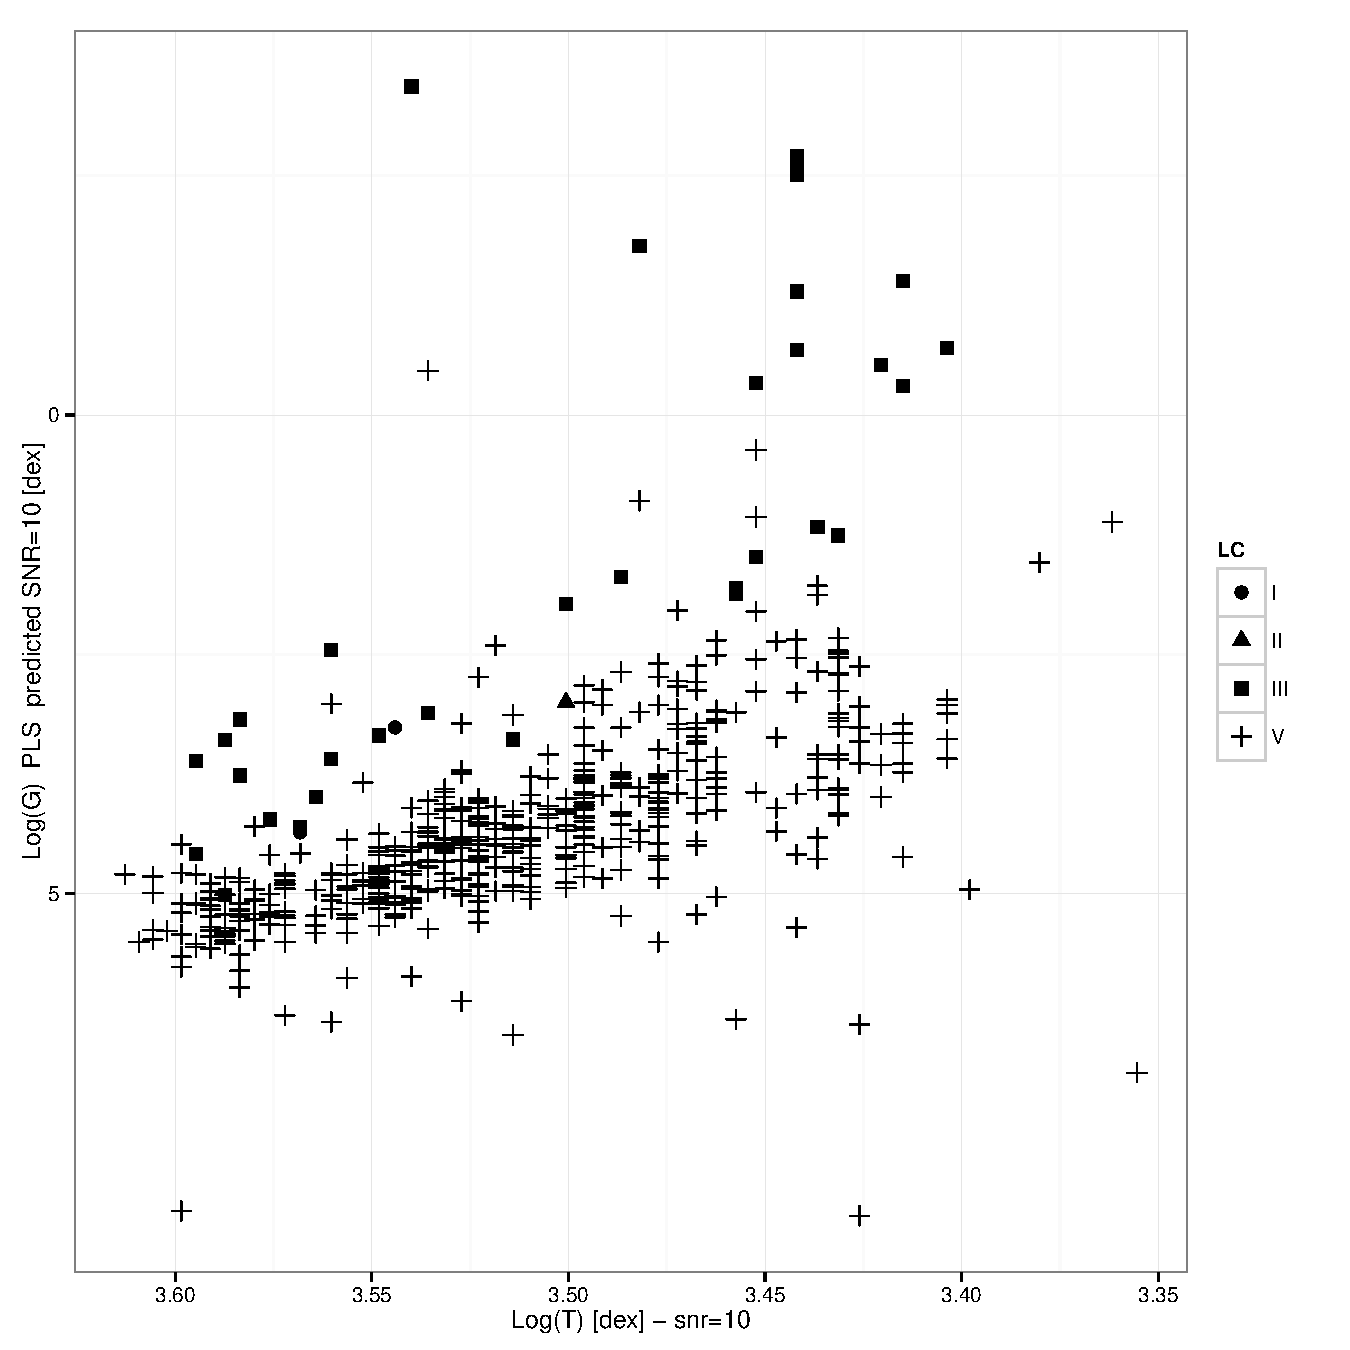
\includegraphics[width=12cm]{figs/ipac_LG_T_PLS_10.pdf}
 \caption{Relationship between $log(T) $ in the x axis 
 and $log(g)$ in the y axis for Partial Least Square model based on the GA provided bandpass features with SNR=$\10$}
 \label{fig:lt_lg_pls}
 \end{center}
\end{figure}

The relationship between the GA predicted Temperature and the one measured by Rojas-Ayala can be 
found in the Figure~\ref{fig:ipac_lt_lt}
\begin{figure}
 \begin{center}
 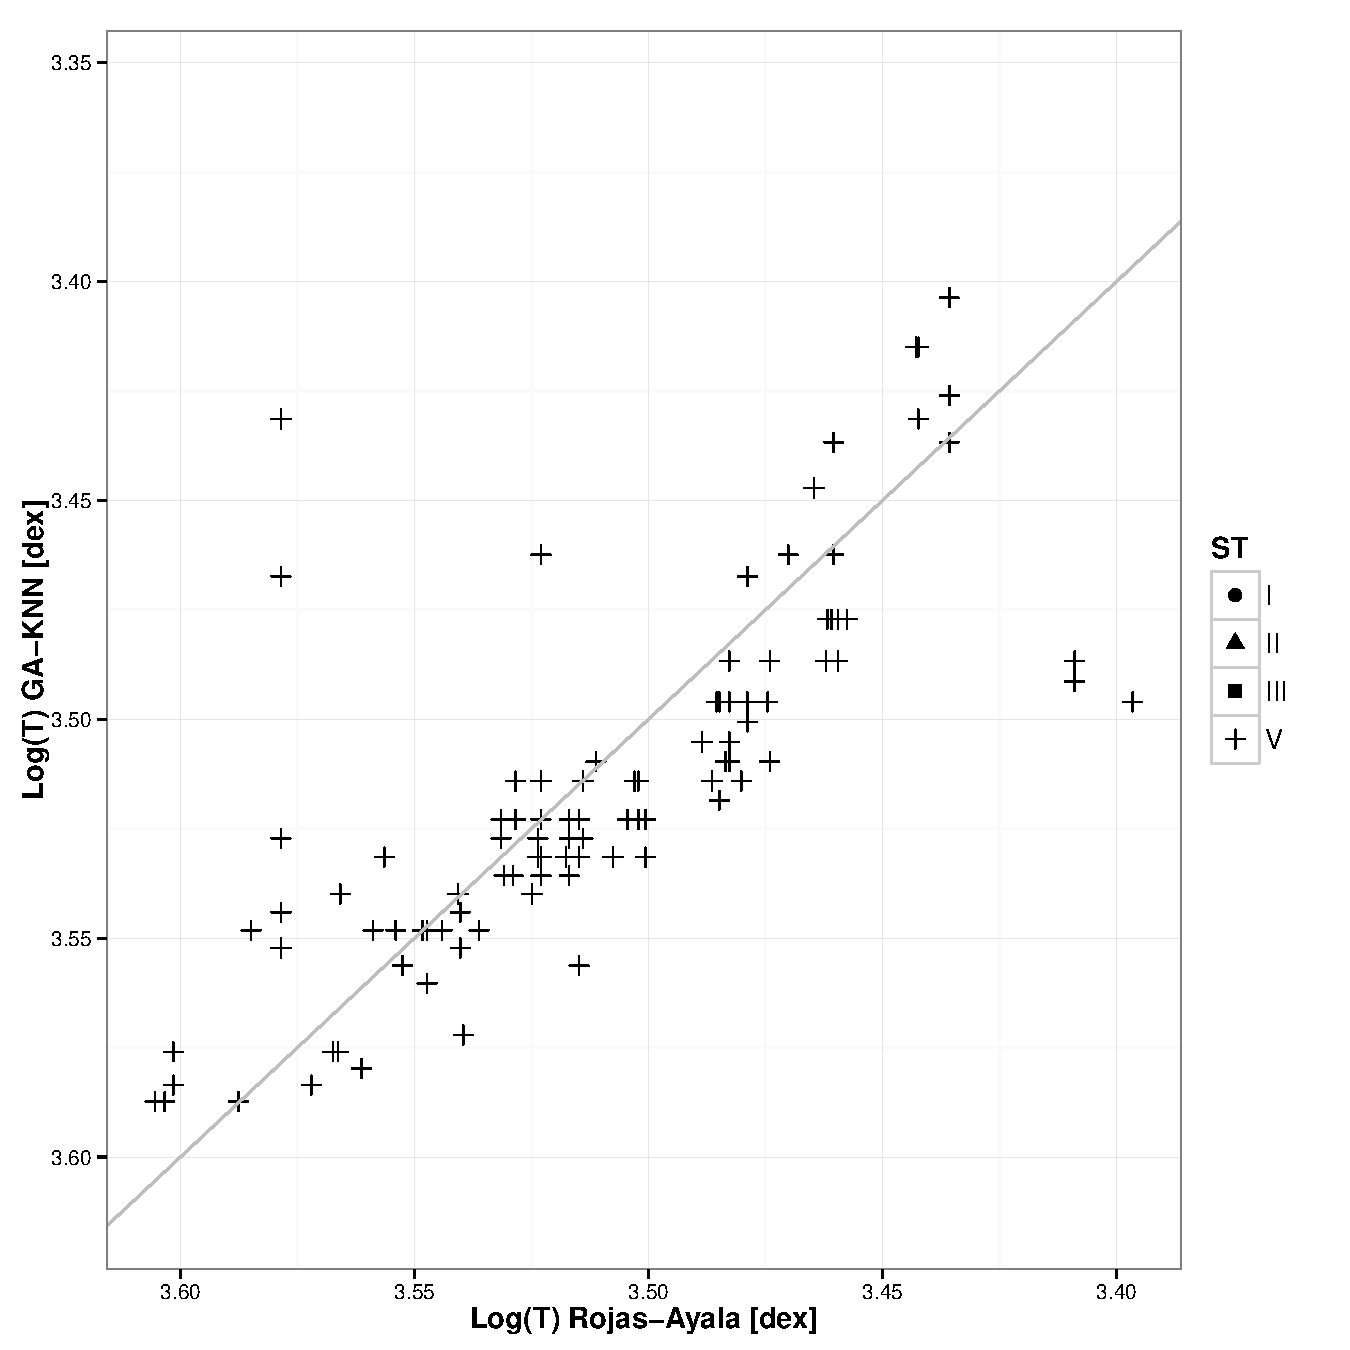
\includegraphics[width=12cm]{figs/ipac_LG_Trojas_Tknn_10.pdf}
 \caption{Relationship between $log(T) from Rojas-Ayala $ in the x axis 
 and $log(T)$ as predicted by KNN with SNR=$\10$}
 \label{fig:ipac_lt_lt}
 \end{center}
\end{figure}

\subsection{Metallicity models} 

Finally, the same analysis is performed for the Metalicty parameter, 
again by considering Temperature as a fixed feature.
In Table~\ref{tab:models_M_rmse} 
we can see the analysis of performance of different classes of
models and cosidering a variety in features. The checks were carried out against 
$Met$ from Neves III.

%
% Metalicidad teórica desde NevesIII para IPAC
%
\ra{1.3}
\begin{table*}\centering
\begin{tabular}{@{}rrrcrrcrr@{}}\toprule
& \multicolumn{2}{c}{$SNR = 10$} & \phantom{ab}& \multicolumn{2}{c}{$SNR = 50$} &
\phantom{ab} & \multicolumn{2}{c}{$SNR = \infty$}\\
\cmidrule{2-3} \cmidrule{5-6} \cmidrule{8-9}
$Regression Models$ & $RMSE$ & $RMDSE$ && $RMSE$ & $RMDSE$     && $RMSE$       & $RMDSE$ \\ \midrule
$\chi^2 BTSettl$    &  0.55    & 0.27   && 0.51 & 0.29 && 0.43  & 0.29 \\
$ ICA+ ppr$         & \bf{0.48} & 0.27 && 0.70  & 0.39 && 0.85  & 0.71 \\
$rf $               & 0.55 & 0.38    && 0.71  & 0.61   && \bf{0.23}  & \bf{0.16} \\
$gbm $              & 0.64 & 0.43 && 0.87  & 0.84  && \bf{0.31}  & \bf{0.23} \\
$ svr $             & \bf{0.46} & \bf{0.26}   && 0.57 & 0.44  && 3.38  & 2.33 \\
$ nnet $            & \bf{0.52} & 0.45      && 0.66 & 0.54  && 2.03  & 1.88 \\
$ knn $             & \bf{0.37}  & 0.28   && 0.99  & 0.78 && 0.56 & 0.32 \\ 
$ mars+ bagging $   & 0.71  & 0.47 && 0.80   & 0.69   && 1.15    & 0.68 \\
$ pls $             & 0.67  & 0.61  && 0.63  & 0.55 && 1.17 & 1.02 \\ 
$Rule Regression $  & \bf{0.47} & 0.29 && 0.50 & 0.36  && 1.18 &  1.18 \\

\bottomrule
\end{tabular}
\caption {RMSE and RMDSE for the various regression models predicting $Met$ [dex].} 
\label{tab:models_M_rmse} 
% \end{center}
\end{table*}



The relationship between the GA predicted Temperature and the one measured by Rojas-Ayala can be 
found in the Figure~\ref{fig:ipac_mt}
\begin{figure}
 \begin{center}
 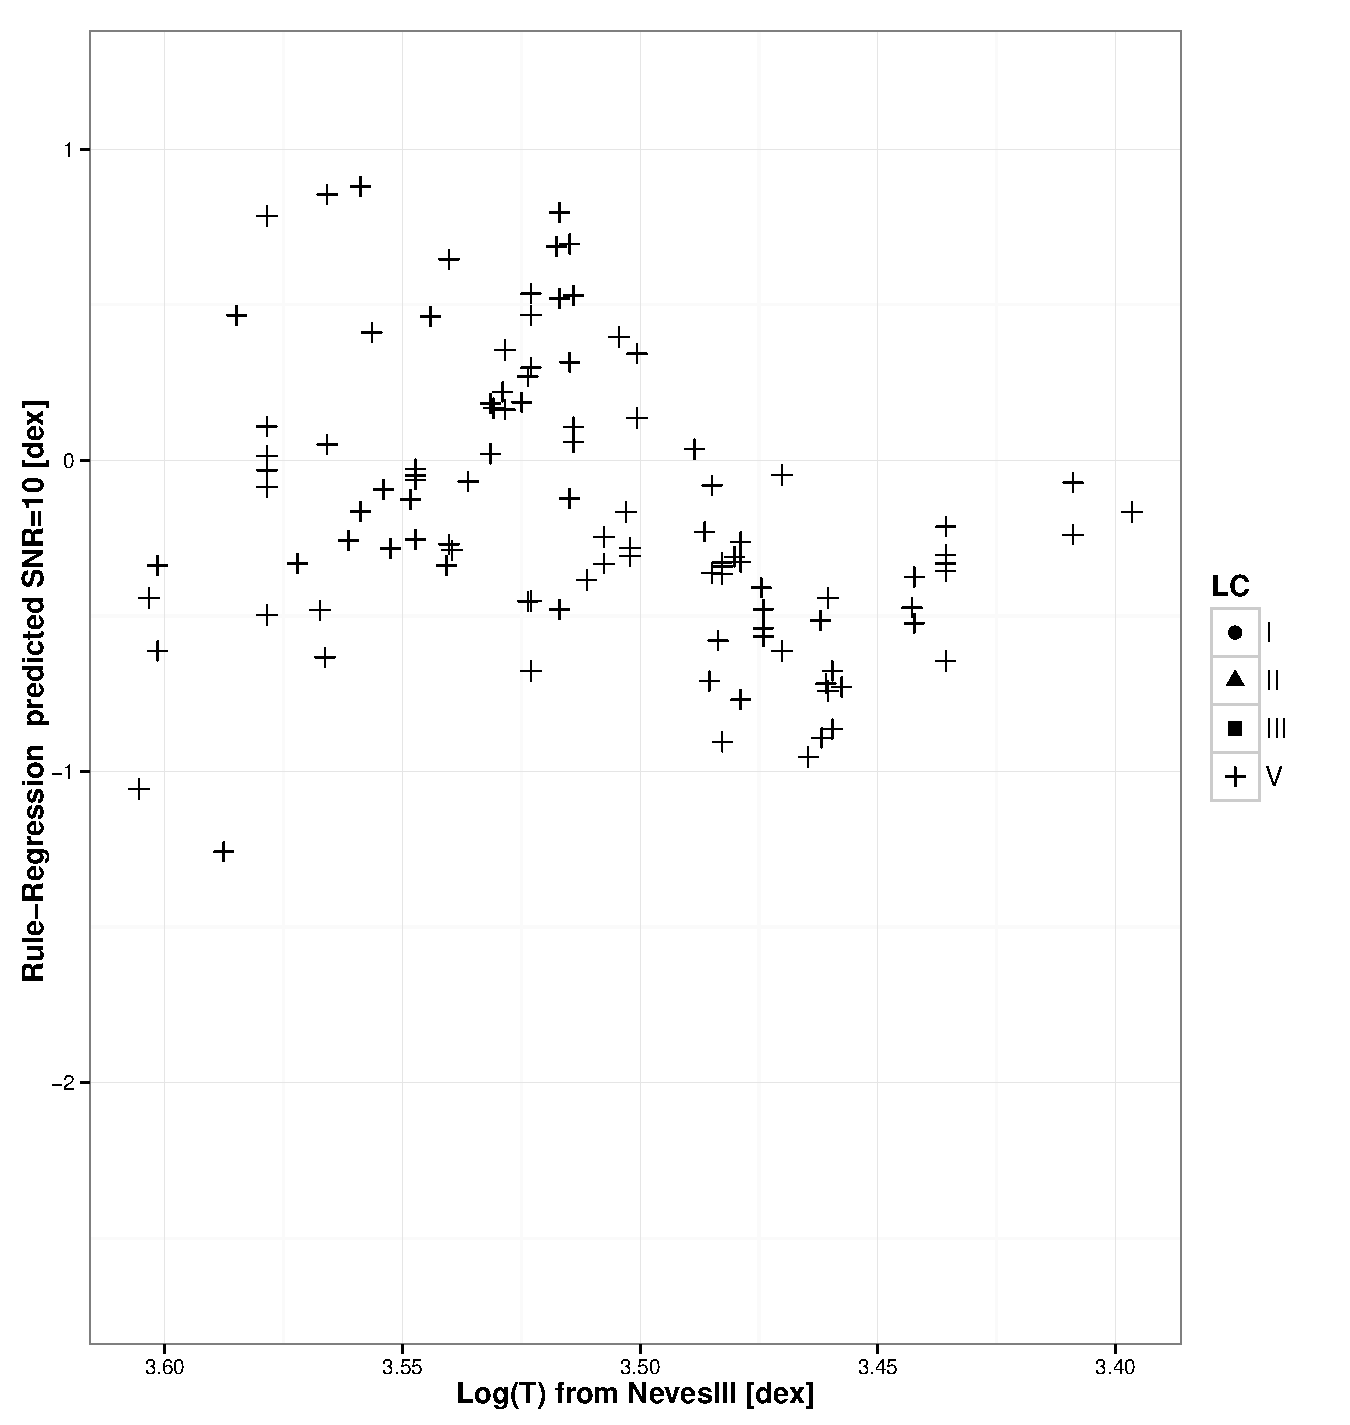
\includegraphics[width=12cm]{figs/ipac_Met_10_NevesIII.pdf}
 \caption{Relationship between $ T from NevesIII $ in the x axis 
 and $ Met $ as predicted by Regression Rules with SNR=$\10$}
 \label{fig:ipac_mt}
 \end{center}
\end{figure}


% In Figure~\ref{fig:M_chi2_50_cesetti} and Figure~\ref{fig:M_GAM_1010_Cesetti} 
% relationships between metalicity predicted by global espectrum estimation 
% and GA feature based estimation against the real values
% provided by \cite{2013A&A...549A.129C} can be observed.

% \begin {figure}
%  \centering
%  \begin{subfigure}{.85\textwidth}
%   \centering
%   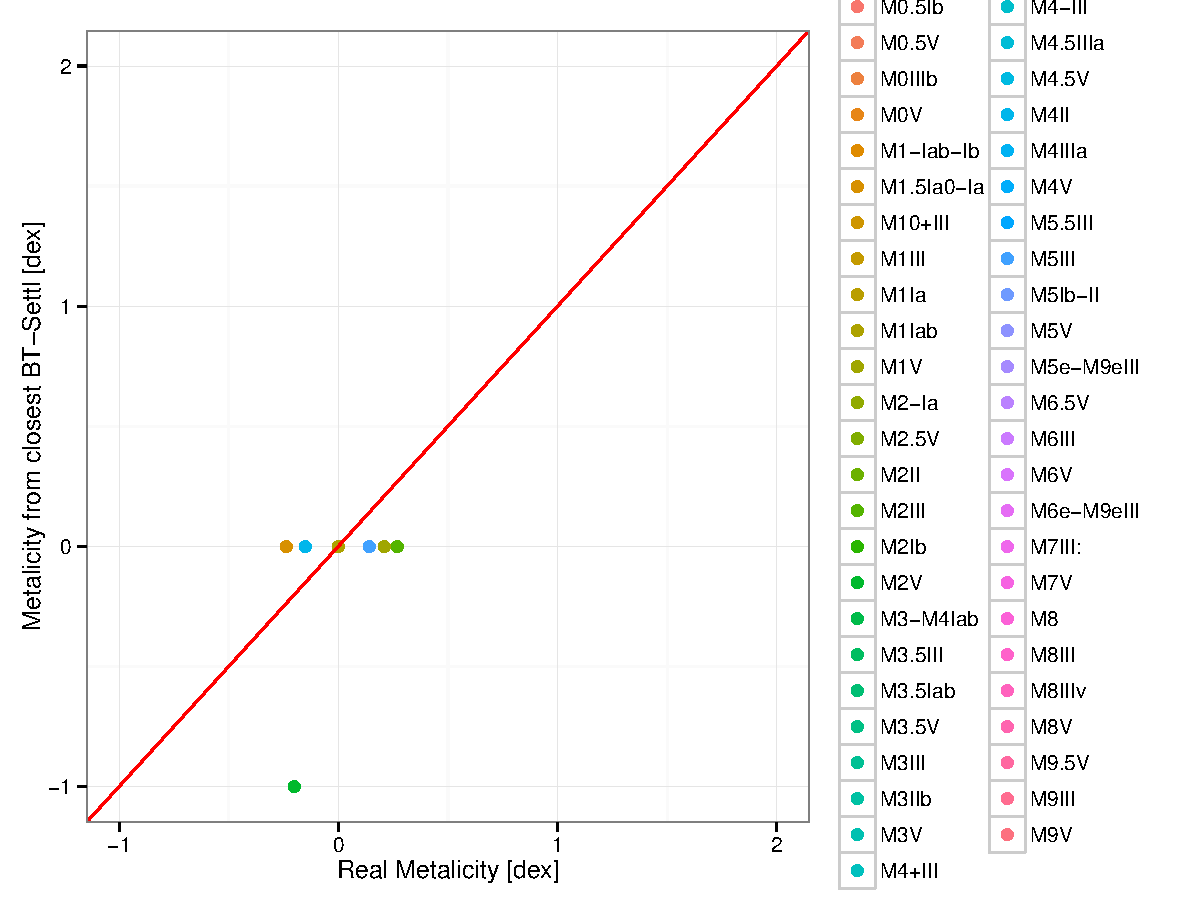
\includegraphics[width=12cm]{figs/M_Chi2_50_Cesetti.pdf}
%   \caption{Comparison between Metalicity estimations from Spectral Subtype 
%  in x axis and the closest BT\_Settl spectra by $\chi^2$ at SNR=$50$ on y-axis}
%  \label{M_chi2_50_cesetti}
%  \end{subfigure}
%   \begin{subfigure}{.85\textwidth}
%   \centering
%   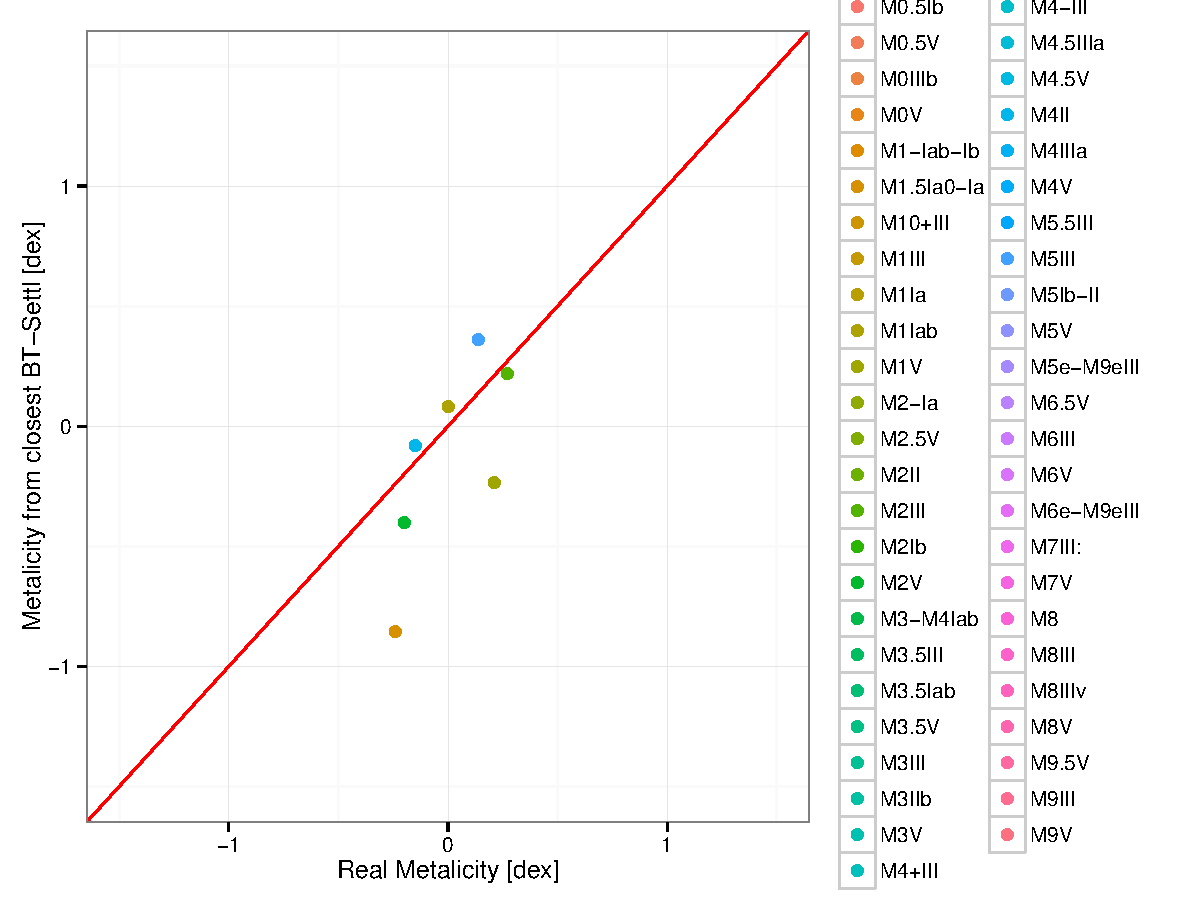
\includegraphics[width=12cm]{figs/M_GAM_1010_Cesetti.pdf}
%   \caption{Comparison between Metalicity estimations from Spectral Subtype 
%  in x axis and the Support Vector Machines for Ga based features trained with BT\_Settl 
%  at SNR=$\infty$ and features for forecasting at SNR=$\infty$ on y-axis}
%  \label{fig:M_GAM_1010_Cesetti}
%  \end{subfigure}
%  \label {fig:comp03}
%  \caption{Performance comparison between the $chi^2$ based selection 
%           and the band oriented features to forecast Log(g)}
% \end {figure}
%
   
   

% De nuevo, el análisis y discusión, función de lo que queramos dejar

